%%%%%%%%%%%%%%%%%%%%%%%%%%%%%%%%%%
%% HA 1 - 03a Phonologie
%%%%%%%%%%%%%%%%%%%%%%%%%%%%%%%%%%

\begin{frame}
\frametitle{Hausaufgabe -- Lösung}
\begin{itemize}
	\item[1.] Ordnen Sie die Artikulationsorte und -organe (Buchstaben) den entsprechenden Bezeichnungen (Klammern) zu.
	
	\begin{minipage}{0.48\textwidth}
		\begin{figure}
			\centering
			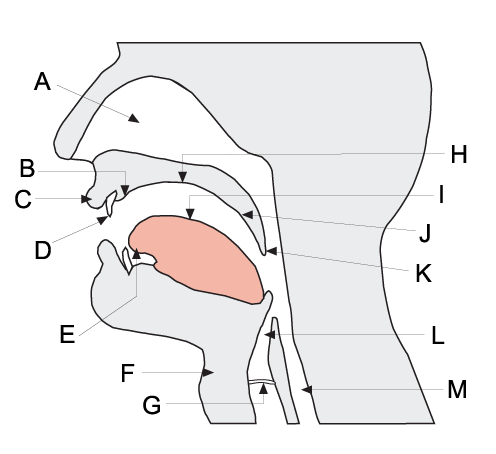
\includegraphics[scale=0.33]{material/04phonoatonomy}
		\end{figure}
	\end{minipage}
	\hfill
	\begin{minipage}{0.4\textwidth}
		
		(\visible<2->{\alertgreen{G}}) Stimmritze (glottal)\\
		(\visible<3->{\alertgreen{F}}) Kehlkopf (laryngal)\\
		(\visible<4->{\alertgreen{B}}) Zahndamm (alveolar)\\
		(\visible<5->{\alertgreen{A}}) Nasenraum (nasal)\\
		(\visible<6->{\alertgreen{H}}) harter Gaumen (palatal)\\
		(\visible<7->{\alertgreen{D}}) Zähne (dental)\\
		(\visible<8->{\alertgreen{J}}) weicher Gaumen (velar)\\
		(\visible<9->{\alertgreen{I}}) Zungenrücken (dorsal)\\
		(\visible<10->{\alertgreen{K}}) Halszäpfchen (uvular)\\
		(\visible<11->{\alertgreen{C}}) Lippen (labial)\\
		(\visible<12->{\alertgreen{E}}) Zungenspitze (apikal)
	\end{minipage}
	
\end{itemize}
\end{frame}


%%%%%%%%%%%%%%%%%%%%%%%%%%%%%%%%
\begin{frame}{Hausaufgabe -- Lösung}
\begin{itemize}
	\item[2.] Welcher Laut passt jeweils nicht in die folgenden Reihen?\\Begründen Sie Ihre Entscheidungen.
	
\begin{exe}
	\exr{ex:03aHA2}
\settowidth\jamwidth{XXXXXXXXXXXXXXXXXXXXXXXt}
	\begin{xlist}
		\ex \textipa{[b]}, \textipa{[z]}, \textipa{[a]}, \textipa{[g]}, \textipa{[v]}, \textipa{[p]}, \textipa{[u]} \loesung{2}{\textipa{[p]} (nicht sth., sondern stl.)}
		\ex \textipa{[t]}, \textipa{[s]}, \textipa{[n]}, \textipa{[\c{c}]}, \textipa{[l]}, \textipa{[d]}, \textipa{[r]} \loesung{3}{\textipa{[ç]} (nicht alveolar, sondern palatal)}
		\ex \textipa{[f]}, \textipa{[s]}, \textipa{[x]}, \textipa{[h]}, \textipa{[r]}, \textipa{[z]}
		\loesung{4}{\textipa{[r]} (kein Frikativ, sondern Vibrant)}
		\ex \textipa{[N]}, \textipa{[m]}, \textipa{[k]}, \textipa{[g]}
		\loesung{5}{\textipa{[k]} (nicht sth., sondern stl.)}\loesung{6}{oder: \textipa{[m]} (nicht velar, sondern labial)}
		\ex \textipa{[m]}, \textipa{[b]}, \textipa{[N]}, \textipa{[p]}
		\loesung{7}{\textipa{[N]} (nicht labial, sondern velar)} \loesung{8}{oder: \textipa{[p]} (nicht sth., sondern stl.)}
	\end{xlist}
\end{exe}
	
\end{itemize}
\end{frame}


%%%%%%%%%%%%%%%%%%%%%%%%%%%%%%%%
\begin{frame}{Hausaufgabe -- Lösung}
\begin{itemize}
	\item[3.] Geben Sie die \textbf{phonologische Repräsentation} der folgenden Wörter und \textbf{verschiedene phonetische Realisierungen} (\zB im Paradigma) an und \textbf{erläutern} Sie anschließend den \textbf{Unterschied} zwischen letzteren.
	
\begin{exe}
	\exr{ex:03aHA3}
	\settowidth\jamwidth{XXXXXXXXXXXXXXXXXXXXXXXXXXXXXXXXXXXXXXt}
	\begin{xlist}
		\ex Dieb
		\loesung{2}{\textipa{/di:b/}: \textipa{[di:p], [di:.bə]} -- Auslautverhärtung des \textipa{/b/} in der Koda}
		\ex König
		\loesung{3}{\textipa{/k\o :nıg/}: \textipa{[k\super h\o:.nıç], [k\super h\o:.nı.gə]} --} \loesung{3}{Spirantisierung des \textipa{/g/} in der Koda}
		\ex eng
		\loesung{4}{\textipa{/εng/}: \textipa{[PεN]}, \textipa{[PENk]} --}
		
		\loesung{4}{ g-Tilgung bzw. (dialektal) Auslautverhärtung}
	\end{xlist}
\end{exe}

\end{itemize}

\end{frame}


%%%%%%%%%%%%%%%%%%%%%%%%%%%%%%%%%
\begin{frame}{Hausaufgabe -- Lösung}

\begin{itemize}
	\item[4.] Bestimmen Sie, ob es sich bei den folgenden Lautkombinationen um Affrikaten handeln kann. Begründen Sie Ihre Entscheidungen.

\begin{exe}	
	\exr{ex:03aHA4}
\settowidth\jamwidth{XXXXXXXXXXXXXXXXXXXXXXXXXXXXXXXXXXXXXXX}
	\begin{xlist}
		\ex \textipa{[kl]} \loesung{2}{keine Affrikate (Zweitglied ist kein Frikativ)}
		\ex \textipa{[pf]} \loesung{3}{Affrikate (Verbindung aus Plosiv und homorganem Frikativ)}
		\ex \textipa{[st]} \loesung{4}{keine Affrikate (Plosiv ist Zweitglied)}
		\ex \textipa{[tr]} \loesung{5}{keine Affrikate (Zweitglied ist kein Frikativ)}
		\ex \textipa{[ts]} \loesung{6}{Affrikate (Verbindung aus Plosiv und homorganem Frikativ)}
	\end{xlist}
\end{exe}

\end{itemize}

\end{frame}


